\documentclass{beamer}\usepackage{graphicx, color}
%% maxwidth is the original width if it is less than linewidth
%% otherwise use linewidth (to make sure the graphics do not exceed the margin)
\makeatletter
\def\maxwidth{ %
  \ifdim\Gin@nat@width>\linewidth
    \linewidth
  \else
    \Gin@nat@width
  \fi
}
\makeatother

\IfFileExists{upquote.sty}{\usepackage{upquote}}{}
\definecolor{fgcolor}{rgb}{0.2, 0.2, 0.2}
\newcommand{\hlnumber}[1]{\textcolor[rgb]{0,0,0}{#1}}%
\newcommand{\hlfunctioncall}[1]{\textcolor[rgb]{0.501960784313725,0,0.329411764705882}{\textbf{#1}}}%
\newcommand{\hlstring}[1]{\textcolor[rgb]{0.6,0.6,1}{#1}}%
\newcommand{\hlkeyword}[1]{\textcolor[rgb]{0,0,0}{\textbf{#1}}}%
\newcommand{\hlargument}[1]{\textcolor[rgb]{0.690196078431373,0.250980392156863,0.0196078431372549}{#1}}%
\newcommand{\hlcomment}[1]{\textcolor[rgb]{0.180392156862745,0.6,0.341176470588235}{#1}}%
\newcommand{\hlroxygencomment}[1]{\textcolor[rgb]{0.43921568627451,0.47843137254902,0.701960784313725}{#1}}%
\newcommand{\hlformalargs}[1]{\textcolor[rgb]{0.690196078431373,0.250980392156863,0.0196078431372549}{#1}}%
\newcommand{\hleqformalargs}[1]{\textcolor[rgb]{0.690196078431373,0.250980392156863,0.0196078431372549}{#1}}%
\newcommand{\hlassignement}[1]{\textcolor[rgb]{0,0,0}{\textbf{#1}}}%
\newcommand{\hlpackage}[1]{\textcolor[rgb]{0.588235294117647,0.709803921568627,0.145098039215686}{#1}}%
\newcommand{\hlslot}[1]{\textit{#1}}%
\newcommand{\hlsymbol}[1]{\textcolor[rgb]{0,0,0}{#1}}%
\newcommand{\hlprompt}[1]{\textcolor[rgb]{0.2,0.2,0.2}{#1}}%

\usepackage{framed}
\makeatletter
\newenvironment{kframe}{%
 \def\at@end@of@kframe{}%
 \ifinner\ifhmode%
  \def\at@end@of@kframe{\end{minipage}}%
  \begin{minipage}{\columnwidth}%
 \fi\fi%
 \def\FrameCommand##1{\hskip\@totalleftmargin \hskip-\fboxsep
 \colorbox{shadecolor}{##1}\hskip-\fboxsep
     % There is no \\@totalrightmargin, so:
     \hskip-\linewidth \hskip-\@totalleftmargin \hskip\columnwidth}%
 \MakeFramed {\advance\hsize-\width
   \@totalleftmargin\z@ \linewidth\hsize
   \@setminipage}}%
 {\par\unskip\endMakeFramed%
 \at@end@of@kframe}
\makeatother

\definecolor{shadecolor}{rgb}{.97, .97, .97}
\definecolor{messagecolor}{rgb}{0, 0, 0}
\definecolor{warningcolor}{rgb}{1, 0, 1}
\definecolor{errorcolor}{rgb}{1, 0, 0}
\newenvironment{knitrout}{}{} % an empty environment to be redefined in TeX

\usepackage{alltt}
\usetheme{Stats}
\setbeamercovered{transparent}
\usepackage{color}
\usepackage{hyperref}
  \hypersetup{
  	colorlinks=true
		linkcolor=black
		}
\usepackage{url}
\usepackage{graphics}
\usepackage{tikz}
\usepackage{booktabs}





%%%%%%%%%%%%%%%%%%%%%%%%%%%%%%%% Title Slide %%%%%%%%%%%%%%%%%%%%%%%%%%
\title[]{Intro to Social Science Data Analysis \\[1cm] Week 12 Lecture: Multivariate Linear Regression \& Presenting Regression Results}
\author[]{
    \href{mailto:gandrud@yonsei.ac.kr}{Christopher Gandrud}
}
\date{\today}


\begin{document}

\frame{\titlepage}

\section[Outline]{}
\frame{\tableofcontents}

%%%%%%%%%% Assignment 4
\section{Assignment 4}
\frame{
  \frametitle{Assignment 4}
  Due: Friday 30 November \\[0.5cm]
  {\Large{Research Design}} \\[0.25cm]
  With your partner plan your research by answering the following questions:
  \begin{enumerate}
    \item What difference or anomaly do you want to explain?
    \item What is your best guess explanation? Draw your best guess in a diagram.
    \item Can you test your hypothesis using data? If so, what data do you need to collect and what tests could you use?
    \item What rival explanations are their?
    \item How could you use data to test whether your best guess or the rival explanations are better? Write this as an \textbf{equation} if possible.
    \item What other factors may influence the relationship you observe?
  \end{enumerate}
{\tiny{Questionnaire from: modified from Cheryl Schonhardt-Bailey}}
}

%%%%%%%%%%% Recap
\section{Recap}
\frame{
	\frametitle{Quick Quiz 1}
{\Large{Interpret the following correlations ($R$):}} \\[0.5cm]
  \begin{itemize}
    \item $R = 0.91$
    \item $R = 0.02$
    \item $R = -0.3$
  \end{itemize}
}

\frame{
  \frametitle{Quick Quiz 2}
  What is a residual?\\[0.5cm]
  Discuss at least \textbf{two} things that residuals are used for in simple linear regression?
}

\frame{
  \frametitle{Quick Quiz 3}
  What assumptions does the linear regression model make?
}

\frame{
  \frametitle{Quick Quiz 4}
  Create a hypothesis test for a linear regression coefficient ($\hat{\beta}$)
}

\frame{
  \frametitle{Quick Quiz 5}
  How do you interpret a linear regression coefficient for a dummy variable?
}

%%%%%% Multiple Linear Regression
\section{Multiple Linear Regression}
\frame{
  \frametitle{Intro to Multiple Linear Regression}
  Last class we learned how to use the tools of simple linear regression to examine the \textbf{bivariate} relationship between a dependent variable and \textbf{one independent} variable. \\[0.5cm]
  What if we want to examine \textbf{multivariate relationships}, i.e. the relationship between a dependent variable and \textbf{multiple} independent variables at the same time? \\[0.5cm]
  In these cases we can use \textbf{multiple linear regression}.
}

\frame{
  \frametitle{Why?}
  \begin{center}
{\Large{\textbf{Why} would we want to examine multiple independent variables at the same time?}}
  \end{center}
}

\frame{
  \frametitle{Minimal criteria for making a causal argument}
  To make a \textbf{probabilistic causal argument}, i.e. ``$X$ caused $Y$" we need to meet \emph{at least} three criteria:
  \begin{itemize}
    \item $X$ is \textbf{statistically associated} with $Y$,
    \item $X$ happens before $Y$ (i.e. \textbf{time order}),
    \item all \textbf{alternative explanations} for the association are ruled out.
  \end{itemize}    
}

\frame{
  \frametitle{Time Order \& Causality}
  {\Large{Linear regression per se can't help us establish time order. \\[0.5cm]
  We need to understand our data to do that. \\[0.5cm]
  We may also need to take measurements at multiple points in time and use more advanced statistical tools than the ones covered in this course.}}
}

\frame{
  \frametitle{Simple Linear Regression \& Causality}
{\Large{Simple Linear Regression is a tool we can use to establish the statistical association between $X$ and $Y$. \\[0.5cm]
  How can we determine how much if at all, the value of $Y$ is actually explained by the value of $X$ and not some other alternative factor(s)?}}
}

\frame{
  \frametitle{Spurious Example}
{\Large{A silly example:}} \\[0.5cm]
  You are interested in what causes expensive fire damage. \\[0.25cm]
  You observe that the most expensive fires have the most fire trucks on the scene. \\[0.25cm]
  Did having more fire trucks cause more damage?
}

\frame{
  \frametitle{Spurious Example}
  Clearly, the \emph{size of the fire} caused both the amount of fire damage and the number of fire trucks that responded. \\[0.5cm]
  There is a \textbf{spurious relationship} between number of fire trucks and fire damage.
}

\frame{
  \frametitle{Spurious Diagram}
  \begin{figure}
    \caption{Spurious Relationship}
    \begin{tikzpicture}
      \vspace{0.5cm}
      %% Nodes
      \node (z) at (0,0) {$Z$};
      \node (x) at (-2, 2) {$X$};
      \node (y) at (2, 2) {$Y$};
      
      %% Arrows
      \draw[->] (z) -- (x);
      \draw[->] (z) -- (y);
      
    \end{tikzpicture}
  \end{figure}
}

\frame{
  \frametitle{Controlling for $Z$}
  If we were able to run an experiment where we \textbf{randomized} the units who are given `treatment' $X$ and those that are not (the `control' group). \\[0.5cm]
  On average the units will have the same values of $Z$. \\[0.5cm]
  We can say that we are \bf{controlling for} $Z$. \\[0.5cm]
  If, after randomization, the association between $X$ and $Y$ still exists, then we have found evidence to rule out alternative explanations.
}

\frame{
  \frametitle{Observational Data}
  However, in many social science situations we cannot run an experiment with randomized control and treatment groups. \\[0.5cm]
  For example, we cannot randomly assign people to live in dictatorships and democracies. \\[0.5cm]
  In these cases we need to use \textbf{statistical control} like \bf{multiple linear regression}.
}

\frame{
  \frametitle{Note:}
  In many cases social scientists actually do conduct randomized experiments. \\[0.5cm]
  For example, the Obama campaign randomized the email messages it sent to people asking for donations. \\[0.5cm]
  Also, there are more advanced statistical techniques that can be combined with multiple linear regression to enhance statistical control. For example, matching.
}

\frame{
  \frametitle{Multi-causality}
  Also, in the social sciences something \emph{rarely has one cause}. \\[0.5cm]
  Instead, phenomenon usually have multiple causes; each making a contribution to the probable value of an outcome. \\[0.5cm]
  Multiple linear regression is a statistical tool that we can use to help identify the \textbf{individual} contribution of some factor to an outcome, \textbf{controlling for} other factors.
}

\frame{
  \frametitle{The Multiple Linear Regression Model}
  An estiamted multiple linear regression model for predictors $x_{1} \ldots x_{p}$:
  \[
  \hat{y} = \alpha + \beta_{1}x_{1} + \beta_{2}x_{2} + \ldots + \beta_{p}x_{p} 
  \]
}

\begin{frame}[fragile]
  \frametitle{Today's Data}
\begin{knitrout}
\definecolor{shadecolor}{rgb}{0.969, 0.969, 0.969}\color{fgcolor}\begin{kframe}
\begin{alltt}
\hlcomment{# Load library}
\hlfunctioncall{library}(openintro)

\hlcomment{# Load data}
\hlfunctioncall{data}(marioKart)

\hlcomment{# Show Variables}
\hlfunctioncall{names}(marioKart)
\end{alltt}
\begin{verbatim}
##  [1] "ID"         "duration"   "nBids"     
##  [4] "cond"       "startPr"    "shipPr"    
##  [7] "totalPr"    "shipSp"     "sellerRate"
## [10] "stockPhoto" "wheels"     "title"
\end{verbatim}
\end{kframe}
\end{knitrout}

\end{frame}

\frame{
  \frametitle{Example Multiple Linear Regression Model}
  Imagine we are interested in what explains the EBay selling price of the game Mario Kart (\texttt{totalPr})? \\[0.5cm]
  We want to see if the duration of the auction in days (\texttt{duration}), whether the game was in used condition (\texttt{condused}), and the number of wheels included in the auction (\texttt{wheels}) impacted the selling price.
}

\begin{frame}[fragile]
  \frametitle{Scatter}
\begin{knitrout}
\definecolor{shadecolor}{rgb}{0.969, 0.969, 0.969}\color{fgcolor}

{\centering 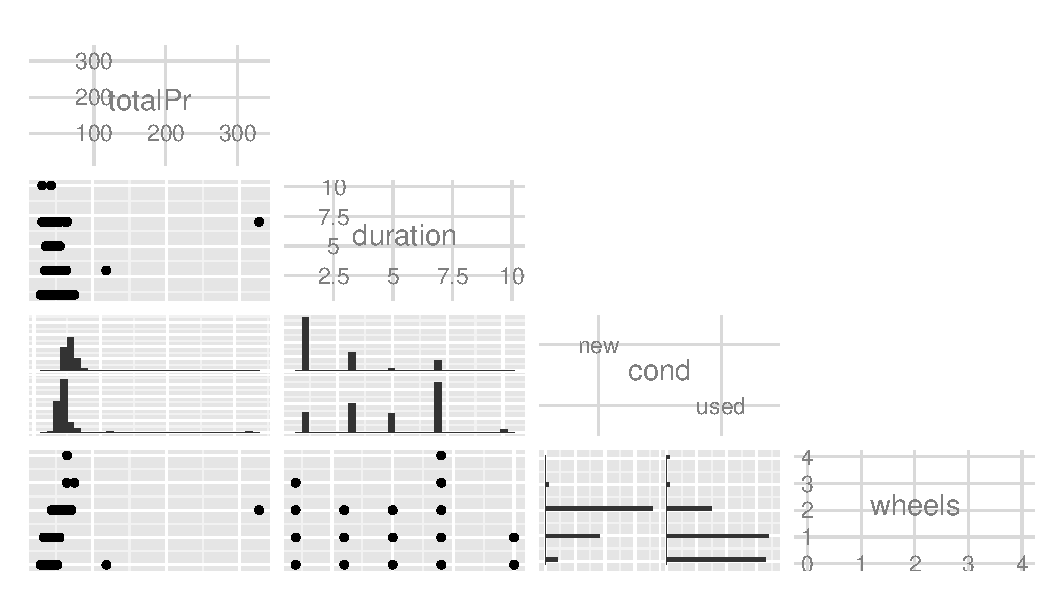
\includegraphics[width=\maxwidth]{figure/Scatter} 

}


\end{knitrout}

\end{frame}

\frame{
  \frametitle{Sum of Squared Residuals}
  Estimating the coefficients and making inferences about them is similar to simple linear regression. \\[0.5cm]
  For example, to find the sum of the squared residals:
  \[
  SSR = \sum^{n}_{i=1} = e^{2}_{i} = \sum^{n}_{i=1} = (y_{i} + \hat{y}_{i})^{2} 
  \]
}

\begin{frame}[fragile]
  \frametitle{Estimation}
  Estimating the $\beta$s by hand in multiple linear regression is very difficult, but it is relatively easy if you let R do the hard work with the \texttt{lm} command:
\begin{knitrout}
\definecolor{shadecolor}{rgb}{0.969, 0.969, 0.969}\color{fgcolor}\begin{kframe}
\begin{alltt}
\hlcomment{# Estimated multivariate linear regression model}
M1 <- \hlfunctioncall{lm}(totalPr ~ duration + cond + 
           wheels, data = marioKart)
\end{alltt}
\end{kframe}
\end{knitrout}

\end{frame}

\begin{frame}[fragile]
  \frametitle{Showing the Coefficient Estimates}
\begin{knitrout}
\definecolor{shadecolor}{rgb}{0.969, 0.969, 0.969}\color{fgcolor}\begin{kframe}
\begin{alltt}
\hlcomment{# Show coefficient point estimates}
M1
\end{alltt}
\begin{verbatim}
## 
## Call:
## lm(formula = totalPr ~ duration + cond + wheels, data = marioKart)
## 
## Coefficients:
## (Intercept)     duration     condused  
##      35.735        0.680       -0.695  
##      wheels  
##      10.455
\end{verbatim}
\end{kframe}
\end{knitrout}

What is the estiatmed linear regression equation?
\end{frame}

\frame{
  \frametitle{Linear Regression Equation}
  \[
  \widehat{\tt{totalPr}} = 35.74 + 0.68\tt{duration} + -0.695\tt{condused} + 10.46\tt{wheels}
  \]
}

\frame{
  \frametitle{Question Linear Regression Equation}
  \[
  \begin{split}
  \widehat{\tt{totalPr}} = & \left 35.74 + 0.68(\tt{duration}) \right. \\
                          & \left + -0.695(\tt{condused}) + 10.46(\tt{wheels}) \right)
  \end{split}
  \]
  What do you estimated will be the total selling price for a Mario Kart auction that was 5 days long, was in new condition, and included 2 wheels?
}

\frame{
  \frametitle{Linear Regression Equation}
  \[
  60.06 = 35.74 + 0.68(5) + -0.695(0) + 10.46(2)
  \]
}


\begin{frame}[allowframebreaks]
  \frametitle{References}
  Crawley, Michael J. 2005. Statistics: An Introduction Using R. Chichester: John Wiley & Sons. Ltd. \\[0.25cm]
  Diaz, David M., Christopher D. Barr, and Mine \c{C}etinkaya-Rundel. 2011. OpenIntro 
  Statistics. 1st ed. \url{http://www.openintro.org/stat/downloads.php}. \\[0.25cm] 
  King, Gary, Michael Tomz, and Jason Wittenberg. 2000. “Making the Most of Statistical Analyses: Improving Interpretation and Presentation.” American Journal of Political Science 44(2): 347–361.
\end{frame}

\end{document}
